\section{Tilstandsmaskin}
\thispagestyle{fancy}

Vi identifiserte tidleg i prosessen at vi hadde eit ønskje om å lage ein tilstandsmaskin som hadde den 
overordna styringa over kvar reaktor. 
Sidan ein SBR tank er prinsipielt oppbygd av forskjellige sekvensar, virka det logisk å lage til ein 
tilstandsmaskin som gjekk igjennom dei forskjellige tilstandane basert på logikk som vart plassert i dei forskjellige tilstandane. 
Med erfaringane vi hadde danna oss om anlegets verkemåte 
kunne vi enkelt tenke oss ei tilstandsmaskin som vart intregert mot dei forskjellige sekvensane i anlegget. 
Tilstandsmaskina tar inn signal i frå dei forskjellige tilstandane i anlegget og avansera til neste 
sekvens når logikken i tilstanden gir signal om at den er ferdig. 


\begin{figure}[htbp]
    \centering
    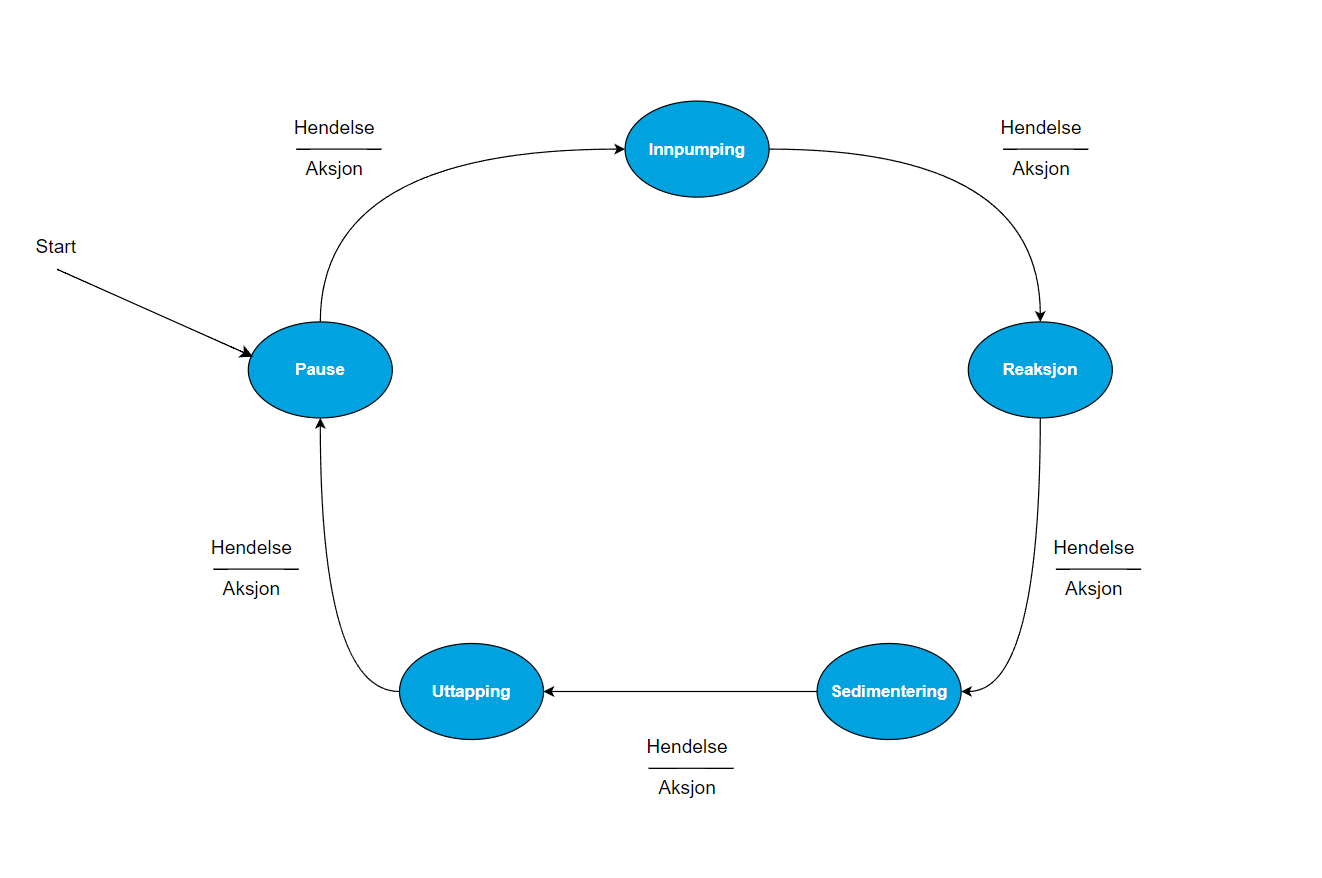
\includegraphics[width=1\textwidth]{Figurar/Tom tilstandsmaskin.png}
    \caption{Tilstandsmaskin prinsipp}\label{fig:Tilstandsmaskin prinsipp}    
\end{figure}

\newpage

